\documentclass[11pt,a4paper,leqno]{article}
\usepackage[utf8]{inputenc}
\usepackage{graphicx}
\usepackage{amsmath}
\author{Wesley}
\title{Notas sobre Redes Neurais}
\begin{document}

\section{Conceitos}
"Sistemas de inteligência artificias contemporâneos não são nada mais do que modelos matemáticos complexos que conseguem aprender uma representação simplificada da realidade, a partir da extração de padrões estatísticos presentes nos dados, que são, por sua vez, extraídos dessa mesma realidade que motiva o aprendizado."

Segundo Tom Mitchel, um software é dito que aprendeu a partir de uma experiência E em alguma tarefa T com uma medida de performance P, se sua performance na tarefa T, medida por P, aumentou sua experiêncie E.

\section{Tipos de Aprendizados}
\subsection{Supervisionado}
No treinamento do modelo são informados os dados para treino (training dataset) e as "respostas corretas" (labels) desse dataset. Neste tipo de treinamento é esperado que a máquina gere um modelo que a partir de um input do dataset ele nos informe o label deste input.
Podemos dividir os problemas de aprendizado supervisionado em duas categorias: \emph{regressão} e \emph{classificação}.

\subsubsection{Regressão}
Tentamos prever o resultado dentro de um output contínuo, ou seja, estamos tentando mapear alguma entrada em uma função contínua.

\subsubsection{Classificação}
Tentamos prever o resultado dentro de outputs discretos, ou seja, estamos tentando mapear alguma entrada em uma classificação discreta.


\subsection{Não-supervisionado}
No treinamento temos pouca ou nenhuma ideia de como nossos resultados deveriam ser. Neste tipo de treinamento derivamos estruturas dos dados onde não sabemos os efeitos das variáveis.
Derivamos as estruturas a partir da clusterização dos dados baseando no relacionamento entre as variáveis.
Não temos feedback nos resultados previstos.


\section{Tipos de Neurônios Artificiais}


\subsection{Perceptron}

Primeiro modelo de neurônio artificial desenvolvido nas decadas de 50 e 60 por Frank Rosenblatt (inspirado no trabalho de Warren McCulloch e Walter Pitts). Atualmente é considerado "ultrapassado".

Recebe um ou mais inputs e produz um output (ativação).
\linebreak
Exemplo de um Perceptron:

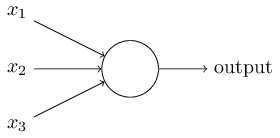
\includegraphics[scale=0.5]{Images/perceptron_model.png} 

Para calcular a ativação do perceptron (o output) utilizamos os pesos (\emph{weights}) associados a cada input ($x_1$, $x_2$, ..., $x_n$) que nada mais são que números reais que expressão a importância do respectivo input para a ativação, ou seja, basicamente pesa as evidências para tomar uma decisão.
Os inputs e outputs são valores binários (0 ou 1), o que o torna nem um pouco sensível.

A ativação do perceptron é determinada por: se a soma dos seus inputs multiplicados pelos seus weights (denotado por \emph{w·x}, onde \emph{w} e \emph{x} são vetores de weights e inputs respectivamente) é maior ou menor que algum valor limite (\emph{threshold}).

Dado um perceptron que receba como input um vetor \emph{x}, temos a fórmula:
\[
  \mbox{output} = \left\{ 
    \begin{array}{ll} 
      0 \ \mbox{se } w\cdot x \leq threshold \\
      1 \ \mbox{se } w\cdot x > threshold
    \end{array}
  \right.
\]

Podemos interpretar o neurônio como um classificador binário, represetado por:
\[ p(y = 1 | x) \]
onde podemor ler como a probabilidade de \emph{x} ser classificado com $y = 1$.

Dado um perceptron que recebe 3 inputs ($x_1, x_2, x_3$), para calcular sua ativação primeiro calculamos seu \emph{weighted input} $z$ (a soma da multiplicação dos inputs por seus weights):
\[
	z = w \cdot x = x_1 * w_1 + x_2 * w_2 + x_3 * w_3
\]
Se $z > threshold$ então output será 1 senão será 0.

Podemos passar o threshold para o outro lado da equação e substituí-lo pelo \emph{bias} do perceptron (\emph{b = -threshold}).

\[
  \mbox{output} = \left\{ 
    \begin{array}{ll} 
      0 \ \mbox{se } w\cdot x + b \leq 0 \\
      1 \ \mbox{se } w\cdot x + b > 0
    \end{array}
  \right.
\]

O \emph{bias} é a medida do quão fácil é ativar o perceptron, ou seja, quão fácil atingir o threshold para produzir o output 1.
Um perceptron com um valor alto no bias é muito fácil ativá-lo e um bias bem negativo torna bem difícil ativá-lo.1

Por fim, podemos definir a função de ativão do perceptron para um input \emph{$x-$} como sendo:

\[
a(x) = \sum_{j=0}^n w_j x_j + b > 0
\]

Variando os \emph{weights} e o \emph{threshold} obtemos diferentes modelos de tomada de decisão para um perceptron e que, quando agrupado, também varia o modelo da rede toda.

Numa rede neural temos vários perceptrons, alguns utilizam como entrada o input do usuário (\emph{input layer}) e outros utilizam como entrada o output de outros perceptrons (\emph{hidden layer}).
\linebreak
Representação Rede Neural com Perceptrons:

http://neuralnetworksanddeeplearning.com/images/tikz1.png



Perceptrons também podem ser usados para calcular funções com lógicas elementares (como AND, OR e NAND).
Um perceptron com duas entradas com weights de -2 cada e um bias de 3, ao receberem entrada de 0 ou 1 conseguem efetuar o NAND das duas entradas.

Para $i_1 = 1$, $i_2 = 0$, temos:
\[ w \cdot x + b =  i_1 * w_1 + i_1 * w_2 + b = 1 * -2 + 0 * -2 + 3 = 1 \]
E para $i_1 = 1$, $i_2 = 1$, temos:
\[ w \cdot x + b = 1 * -2 + 1 * -2 + 3 = -1 \]

Os perceptrons conseguem simular qualquer operação lógica ou circuitos delas. E por esses circuitos serem universais na computação, isso implica que os perceptrons também são universais.
Porém, por causas dos \emph{weights} e \emph{bias} as soluções podem ser tunáveis, podemos alterar os valores para produzir os resultados aceitáveis. E com algoritmos de aprendizado é possível que essas variáveis sejam tunadas automaticamente conforme os treinos.



\subsection{Neurônios Sigmoid}

Similares aos perceptrons, porém modificado para que pequenas mudanças nos weights e bias cause pequena mudança no output. Pois um perceptron ao sofrer uma pequena mudança no weight ou bias pode inverter completamente seu output.

Essa pequena mudança facilita e muito o autoaprendizado, pois permite uma evolução passo a passo, sem que a coisa saia do controle.

Os Sigmoids possuem a mesma estrutura dos perceptrons, porém seus inputs e outputs são valores reais entre 0 e 1 pois utilizam a função de ativação \emph{sigmoid}.

Notação utilizada:

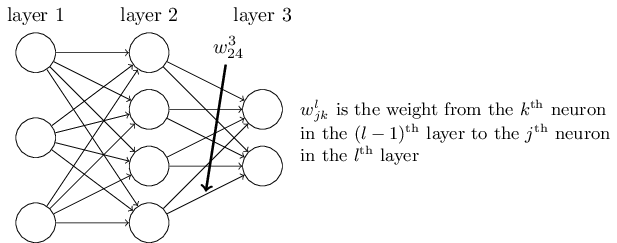
\includegraphics[scale=0.5]{Images/neural_network_notation.png} 


A ativação (output) de um sigmoid é dada pela função de ativação sigmoid sobre seu weighted input $z$:
\[
	z^l_j = \sum_k w^{l}_{jk} a^{l-1}_k + b^l_j
\]
\[
  a^{l}_j = \sigma (z^l_j)
\]
onde $a^l_j$ representa a ativação do neurônio $j^{th}$ na camanda $l^{th}$, $w^l_{jk}$ representa o weight do neurônio $j^{th}$ da camada $l^{th}$ com o neurônio $k^{th}$ da camada $(l-1)^{th}$, $a^{l-1}_k$ representa o output do neurônio $k^{th}$ da camada $(l-1)^{th}$ (ou no caso da primeira camada representa o input), $b^l_j$ representa o bias do neurônio $j^{th}$ da camada $l^{th}$, e $\sigma$ é a função \emph{sigmoid} (as vezes referenciada função logística).

Podemos representar essa expressão utilizando matrizes:
\[
 a^l_j = \sigma(w^l_j \cdot x^{l-1} + b^l_j)
\]
onde $x^{l-1}$ é o vetor de input (outputs da camada anterior ou input da primeira camada), $w^l_j$ é o vetor de weights do neurônio $j^{th}$ da camada $l^{th}$, $b^l_j$ é o bias do neurônio $j^{th}$ da camada $l^{th}$.

Para representarmos o output de todos os neurônios de uma determinada camada podemos simplificar removendo os índices $j$:
\[
 a^l = \sigma(w^l \cdot x^{l-1} + b^l)
\]


A função de ativação sigmoid ($\sigma$), as vezes referenciada função logística, é definida por:
\[
 \sigma(z) \equiv \frac{1}{1+e^{-z}}
\]
Se $z$ for um vetor a função sigmoid retorna um vetor de outputs, um output para cada item do vetor de entrada, conforme:
\[ \sigma(v)_j = \sigma(v_j) \]

Quandos o valor de \emph{w·x + b} é muito negativo ou muito positivo, os outputs são bem próximos de 0 e 1, respectivamente, assim como nos perceptrons. Porém quando o valor tem um tamanho modesto a saída é diferente pois varia entre 0 e 1, e essa pequena mundaça causa a forma em S da função quando plotada (ao contrário da função do perceptron que praticamente tem formato digital).

Abaixo segue o formato geral da função:\\
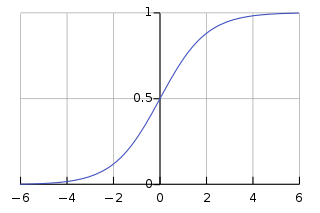
\includegraphics[scale=0.4]{Images/conjunto_imagem_funcao_ativacao_sigmoid.png} 

Essa curva suave em S permite que pequenas mudanças no weight ou no bias cause pequena mudança no output.
A variação do output é uma função linear das variações de weight e bias. Essa lineariedade facilita a escolha/descoberta dessas variações para atingir a variação desejada no output.
\[
  \Delta \mbox{output} \approx \sum_j \frac{\partial \, \mbox{output}}{\partial w_j}
  \Delta w_j + \frac{\partial \, \mbox{output}}{\partial b} \Delta b,
\]


\newpage
\section{Arquitetura de uma Rede Neural}

Como visto, o neurônio perceptron e sigmóid realizam apenas uma classificação linear binária (linear regression classifier), então função apenas para resolução de problemas onde o modelo pode ser dividido de forma linear (como em um gráfico).
Com um rede de neurônios artificiais podemos fazer uma classificação não-linear, podendo classificar um input como sendo de uma determinada classe.

Para cada classe que queremos multiplicar teremos um neurônio artificial na última camada da rede para nos informar a probabilidade daquele input ser daquela classe.
Podemos representar a saída da rede neural como:
\[
	p(y = c | x)
\]
onde \emph{c} é um vetor com as probabilidades do input \emph{x} percencer a uma determinada classe (o index do vetor representa uma das classes em $\{ 1, 2, ..., C \}$ onde).

A rede neural é divida em várias camadas compostas por vários neurônios artificiais, a camada de neurônios mais a esquerda é chamada input layer, a camada mais a direita é chamada output layer e as camadas do meio são chamadas de hidden layer.
As funções de ativação dos neurônios podem variar de camada para camada, o que proporciona um maior poder à rede neural.

Redes neurais com várias camadas são chamadas multilayer perceptrons ou \emph{MLP}, independente se forem formadas por perceptrons ou neurônios sigmoid.

O design das input e output layers são bem diretos, diretamente ligadas ao design do problema (se for para identificar se numa imagem existe o número 1, então temos a quantidade de inputs igual à resolução da imagem e um output para informar se tem ou não o número na imagem.
	
O design das hidden layers é uma arte e existem poucas regras de ouro. Pesquisadores tem desenvolvidos vários design heurísticos que ajudam a obter determinado comportamento (por exemplo, determinar a relação de quantidade de hidden layeres com o tempo de treino).

Uma rede neural é composta por um conjunto de hiperparâmetros que pode definir o quão bom será na tarefa e o quanto o aprendizado irá ajudar. Porém não podemos ter certeza disso, para encontrar os valores ideias precisamos, a partir de uma inicialização aleatória dos parâmetros \emph{weights} e \emph{biases}, testar a variação deses hiperparâmetros.
Alguns deles:
\begin{itemize}
\item $\eta$ ou learning rate: é a taxa de aprendizado da NN, ela determina o "tamanho" do passo que daremos a cada ciclo do aprendizado, dependendo do método escolhido para aprendizado.
\item qtde. camadas: a quantidade de camadas da nossa NN define o quão abstrata nossa rede pode ser, pois provavelmente cada camada estaria especializada em uma tarefa, e também pode definir o quão demorado será o treinamento (uma NN com muitas camadas pode levar muito tempo para treinamento).
\item \emph{mini-batch}: define o tamanho da divisão que faremos nos dados para que possamos ter um aprendizado mais rápido pois estamos fazendo pequenos treinamentos com cada conjunto.
\item \emph{epoch} (épocas): quantidade de ciclos que faremos nos dados durante o treinamento (sempre escolhendo os mini-batch de forma aleatória).
\end{itemize}

Uma NN não é fácil de debugar pois quase sempre não sabemos a melhor forma de inicializar seus parâmetros e durante nossas variações não podemos ter certeza o impacto da variação de cada hiperparâmetro na nossa NN.


Durante o treinamento a rede pode gerar uma representação abstrata dos dados e essa representação é utilizada para realizar uma previsão ou classificação. Essa abstração é difícil de se prever de como fica arquitetada entre as layers da rede (níveis hierárquicos de abstração). Como exemplo, imagine uma rede treinada para identicar objetos, pode ser que as primeiras camadas fiquem responsáveis por identificar linhas e pontos nas formas, as camadas seguintes fiquem responsável por identificar formas mais abstratas como formas geométricas, e assim por diante. \linebreak
Podemos explorar o que cada camada está fazendo através do aumento dos valores dos seus \emph{weights} e \emph{biases} e ver o output dela (vide Deep Dream).

Essa estrutura de IA que utilizaca camadas para representação é chamada \textbf{Deep Learning}.



\subsection{Redes Neurais Feedforward}
São redes que os outputs de uma camada são os inputs da próxima camadas.
Nelas não existe loop, ou seja, nenhuma camada produz outputs que são inputs de uma camada anterior.
Os algoritmos de aprendizado são mais poderosos que os do RNN.




\subsection{Redes Neurais Recorrente (RNN)}
Possuem loops, ou seja, uma camada a frente produz output que serve de input para uma camada anterior.

A ideia neste modelo é ter neurônios que ativam somente durante um tempo limitado antes de se tornarem ociosos. Essa ativação estimula outros neurônios que também são ativados por um tempo limitado. Criando assim uma cascata de ativação assíncrona, o que não cria loops.

Os seus algoritmos de aprendizado não são tão poderosos quanto os do Feedforward porém seu modelo de funcionamento está mais próximo ao do cérebro do que o Feedforward está.


\newpage
\section{Algoritmos}

\subsection{Univariate Linear Regression}
É um modelo para modelar o relacionamento entre uma variável numérica \emph{y} (variável dependente) e uma variável explicativa (uma feature, variável independente) \emph{x}.
A partir de uma dataset de treinamento, utilizamos um algoritmo de aprendizado para poder obter uma função hipótese que mapeie \emph{x's} para \emph{y's}.
\[h:X \rightarrow Y\]
A função h tem o seguinte formato:
\[ h_\theta(x) = \theta_0 + \theta_1 x \]
onde $\theta_i$'s são parâmetros do modelo.

Para obter essa função \emph{h} é executado um processo estatístico chamado \emph{Análise de Regressão (regression analysis)} para estimar o relacionamento entre as variáveis independentes \emph{x's} e a variável dependente \emph{y}.
Para obter a função precisamos encontrar os valores $\theta_i$ para que $h_\theta (x^{(i)} \simeq y^{(i)}$.

O ato de tentar encontrar os valores ideais para $\theta_i$ é um problema de minimização, sendo assim, temos várias funções que podemos usar.


\subsubsection{Função de Custo Squared Error Function}
Para minimizar $\theta_i$ podemos usar a função Squared Error Function que mede a acurácia da função hipótese $h$ através da diferença média de todos os resultados gerados pela hipótese utilizando os inputs \emph{x's} e os outputs esperados \emph{y's} (diferença média entre o valor previsto e o valo real).

\[
Minimizar \ \theta_0, \theta_1 \rightarrow C (\theta_0, \theta_1) = \frac{1}{2m} \sum_{i=1}^m ( h_\theta (x^{(i)}) - y^{(i)}) ^ 2
\]

\subsubsection{Gradiente Descendente}
Para nos ajudar a minimizar a função usamos o algoritmo gradiente descendente para encontrar o local mínimo da função de custo.
Para fazer isso utilizamos o gradiente da função para nos orientarmos até o local mínimo.
Os passos para implementação:
\begin{itemize}
\item iniciar $\theta_i$ com valores aleatórios
\item atualizar constantemente $\theta_i$ para reduzir $C(\theta_0, \theta_1)$ até que não haja mais atualizações (encontrou o local mínimo da função)
\end{itemize}

Para atualizar os parâmetros da função $C$ utilizamos as derivadas parciais de cada parâmetro da função ($\theta_0$ e $\theta_1$):
\[
\theta_0 := \theta_0 - \eta \frac{1}{m} \sum\limits_{i=1}^{m} (h_\theta(x^{(i)}) - y^{(i)})
\] \[
\theta_1 := \theta_1 - \eta \frac{1}{m} \sum\limits_{i=1}^{m} (h_\theta(x^{(i)}) - y^{(i)}) \cdot x^{(i)}
\]
onde $\eta$ é a fator do passo na iteração (nosso learning rate).




\subsection{Multivariate Linear Regression}
É uma versão da Linear Regression com várias variáveis.\\
Permite modelar o relacionamento entre uma variável numérica \emph{y} e várias variáveis explicativas (features de 0 a $n$) \emph{x's}.
A função hipótese tem o formato:
\[ h_\theta(x) = \theta_0 + \theta_1 x_1 + ... + \theta_n x_n \]

Por conveniência de implementação, assumiremos todo $x_0^{(i)} = 1$, então podemos reescrever a função hipótese como:
\[ h_\theta(x) = \theta_0 x_0 + \theta_1 x_1 + ... + \theta_n x_n \]
E ainda:
\[ h_\theta(x) = \sum_{j=0}^n \theta_j x_j \]

Utilizando matrizes, podemos escrever as features X e parâmetros $\Theta$:
\[
X = \begin{bmatrix}
	x_{0} \\
	x_{1} \\
	\vdots \\
	x_{n}
 \end{bmatrix}
\]
 
\[
\Theta = \begin{bmatrix}
	\theta_{0} \\
	\theta_{1} \\
	\vdots \\
	\theta_{n}
 \end{bmatrix}
\]

E escrever função hipótese como:
\[ h_\theta(x) = \Theta^T X \texttt{ ou } h_\theta(x) = X \Theta \]



\subsubsection{Função de Custo Squared Error Function}
Função de custo é a mesma da Linear Regression, porém na notação usamos os vetores X e $\Theta$ para simplificar.

\[
Minimizar \ \Theta \rightarrow C (\Theta) = \frac{1}{2m} \sum_{i=1}^m ( h_\theta (x^{(i)}) - y^{(i)}) ^ 2
\]

Na forma vetorizada podemos escrever como:
\[
Minimizar \ \Theta \rightarrow C (\Theta) = \frac{1}{2m} (X \Theta - y)^T (X \Theta - y)
\]

\subsubsection{Gradiente Descendente}
Equivalente à Linear Regression, para minimizar a função de custo $C$ utilziamos a derivada parcial de cada parâmetro do vetor $\Theta$ conforme:
\[
\theta_j := \theta_j - \eta \frac{1}{m} \sum\limits_{i=1}^{m} (h_\theta(x^{(i)}) - y^{(i)}) \cdot x_j^{(i)}
\]

Nota: como assumimos $x_0^{(i)} = 1$ podemos utilizar apenas uma fórmula aqui.



\subsection{Classificação com Regressão Logística}
Aplicamos esse algorítmo em problemas de classificação, que são parecidos com problemas de regressão com a exceção que queremos prever um conjunto de valores discretos.
Nele fazemos a predição da classe \emph{y} em um conjunto de valores discretos.

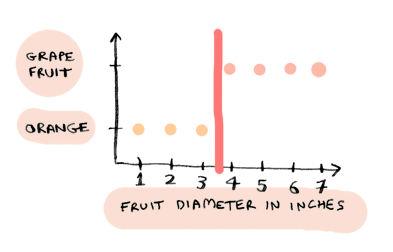
\includegraphics[scale=0.5]{Images/logistic_regression_plot_fit.png} 

Acima temos um exemplo de um modelo que classifica as flutas laranja na classe 0 e as uvas na classe 1, onde o threshold tem valor de 3,5.

No caso de um classificado binário, onde queremos classificar um input \emph{x} como 0 ou 1, teremos $y \in \{0, 1\}$.
Dizemos que $0$ é a \emph{classe negativa} e $1$ é a \emph{classe positiva}.

Para que nosso modelo tenha um \emph{output y} entre os valores discretos das classes utilizamos uma função logística que defina os limites do nosso output.
Com isso, nossa função hipótese terá o seguinte formato:
\[ h_\theta (x) = g(\Theta^T x) \]
No caso de um classificador binários podemos usar a \emph{função sigmóid} onde nosso output será entre 0 e 1.
A função sigmóid tem o seguinte formato:
\[ g(z) = \dfrac{1}{1 + e^{-z}} \]
onde $z = \Theta^T x$. E ela tem a seguinte propriedades:
\begin{eqnarray*}
	z=0, e^{0}=1 \Rightarrow g(z)=1/2 \\
	z \to \infty, e^{-\infty} \to 0 \Rightarrow g(z)=1 \\
	z \to -\infty, e^{\infty}\to \infty \Rightarrow g(z)=0
\end{eqnarray*}

Podemos ver que $g(z) \geq 0.5$ quando $\Theta^Tx \geq 0$.

Então definimos um \emph{threshold} (aqui no caso $0.5$) para classificar nosso output $h_\Theta(x)$:
\[
  \left\{ 
    \begin{array}{ll} 
      \mbox{se } h_\theta(x) \geq threshold \rightarrow y = 1 \\
      \mbox{se } h_\theta(x) < threshold \rightarrow y = 0
    \end{array}
  \right.
\]

Podemos finalizar com:
\begin{align*}
	\Theta^T x \geq 0 \Rightarrow y = 1 \\
	\Theta^T x < 0 \Rightarrow y = 0
\end{align*}

Podemos interpretar o output como a probabilidade de $y = 1$ dado input x parametrizado por $\Theta$:
\[ h_\theta(x) \rightarrow P(y = 1 | x; \Theta) \]

Os limites da decisão define as áreas do gráfico onde $y = 0$ e $y = 1$, esses limites são definido pela forma da nossa função hipótese quando plotado no gráfico.

\subsubsection{Função de Custo Logística}
Não podemos utilizar a Square Error Function pois o gráfico será não-convexo (terá formato de onda) pois não convergeremos para o local mínimo.

Usamos uma função de custo logística:
\begin{align*}
& C(\Theta) = \frac{1}{m} \sum_{i=1}^m Cost(h_\theta(x^{(i)}), y^{i}) \\
& Cost(h_\theta(x^{(i)}), y^{i}) = -log(h_\theta(x)) \ \ \ \ \ \ \text{ se y = 1} \\
& Cost(h_\theta(x^{(i)}), y^{i}) = -log(1 - h_\theta(x)) \ \text{ se y = 0}
\end{align*}

Nela temos as seguintes propriedades:
\begin{align*}
	& \mathrm{Cost}(h_\theta(x),y) = 0 \text{ se } h_\theta(x) = y \\
	& \mathrm{Cost}(h_\theta(x),y) \rightarrow \infty \text{ se } y = 0 \; \mathrm{e} \; h_\theta(x) \rightarrow 1 \\
	& \mathrm{Cost}(h_\theta(x),y) \rightarrow \infty \text{ se } y = 1 \; \mathrm{e} \; h_\theta(x) \rightarrow 0
\end{align*}

Podemos escrever a função de custo na forma compacta:
\[
C(\Theta) = - \frac{1}{m} \displaystyle \sum_{i=1}^m [y^{(i)} \log(h_\theta(x^{(i)})) + (1 - y^{(i)}) \log(1 - h_\theta(x^{(i)}))]
\]

Abaixo temos a plotagem das função de custo $C$ em função da classe prevista para os casos em que $y = 0$ e $y = 1$, note que devido à função $Cost(h_\theta(x^{(i)}), y^{i})$ que usamos para cada classe temos diferentes formas.

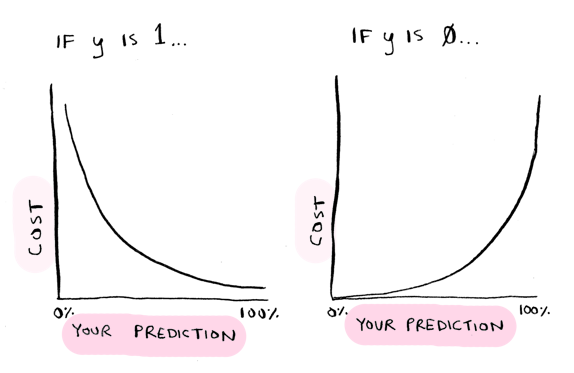
\includegraphics[scale=0.5]{Images/logistic_regression_plot_cost_function.png} 


\subsubsection{Gradiente Descendente}
Os passos de aplicaçao são iguais ao da Linear Regression porém divido a mudança da função de custo teremos apenas uma mudança na derivação utilizada.
\[
\theta_j = \theta_j - \eta \frac{\partial}{\partial \theta_j} C(\Theta)
\]
onde
\[
\frac{\partial}{\partial \theta_j} C(\Theta) = \frac{1}{m} \sum_{i=1}^m (h_\theta(x^{(i)}) - y^{(i)}) x_j^{(i)}
\]
Então teremos no fim:
\[
\theta_j := \theta_j - \frac{\alpha}{m} \sum_{i=1}^m (h_\theta(x^{(i)}) - y^{(i)}) x_j^{(i)}
\]
alpha
Podemos reescrever na forma vetorizada:
\[ h = g(X \Theta) \]
\[
C(\Theta) = \frac{1}{m} (-y^T \log(h) - (1 - y)^T \log(1 - h))
\]
E a atualização vetorizada:
\[
\Theta = \Theta - \frac{\eta}{m} x^T (g(X\Theta) - \vec{y})
\]
	
\newpage
\section{Aprendizado}

\subsection{Função de Custo (ou perda)}
Utilizamos uma função de custo para podermos verificar o quão próximo os outputs da rede neural estão dos resultados esperados para um conjunto de dados de treinamento.

O resultado dessa função mostra o quão bom é o nosso algoritmo, quanto mais próximo do 0 melhor o nosso algoritmo se torna, pois 0 significa que todos os outputs são iguals ao output esperados.

Então para que nosso modelo se aproxime dos resultados esperados precisamos minimizar os parâmetros (weights e biases) para que o resultado da função de custo se aproxime de 0.
\[
Minimizar \ w, b \rightarrow C(w, b) \simeq 0
\]

O ato de tentar encontrar os valores ideais para os parâmetros é um problema de minimização, sendo assim, temos vários métodos que podemos usar.


\subsubsection{Quadratic Cost}

Para calcular o erro dos parâmetros atuais podemos usar a função Squared Error Function (também conhecida por \emph{mean squared error} ou MSE) que mede a acurácia da função hipótese $h$ através da diferença média de todos os resultados gerados pela hipótese utilizando os inputs \emph{x's} e os outputs esperados \emph{y's} (diferença média entre o valor previsto e o valo real).

\[
C(\Theta) \equiv \frac{1}{2n} \sum_x (y(x) - h(x))^2.
\]

Onde $\Theta$ é o vetor com os parâmetros (weights e biases), \emph{n} é a quantidade de elementos do treinamento, \emph{y(x)} é o output esperado dado o input \emph{x} e \emph{h(x)} é o output do nosso algoritmo dado input \emph{x} com o weight \emph{w} e bias \emph{b}.

Nota: A média é dividida ($\frac{1}{2}$) como conveniência para o cálculo do gradiente descendente, onde a derivada da função da potência de 2 será cancelada pela divisão.


\subsubsection{Logistic Cost}
Utilizamos a função de custo logistica nos casos de classificação onde temos uma função de squashing (em que comprimimos os resultados em um conjunto discreto) pois ela é convexa nesses casos.
\[
C(\Theta) = - \frac{1}{m} \displaystyle \sum_{i=1}^m [y^{(i)} \log(h_\theta(x^{(i)})) + (1 - y^{(i)}) \log(1 - h_\theta(x^{(i)}))]
\]

\subsection{Minimização da Função de Custo}
Para minimizar nossa função de custo podemos utilizar alguns algoritmos:
\begin{itemize}
\item Gradient Descent
\item Conjugate Gradient
\item BFGS
\item L-BFGS
\end{itemize}

\subsection{Gradient Descent}

Para minimizar a função de custo $C$ precisamos encontrar os \emph{weights} e \emph{biases} ideais para o nossa rede. E para encontrar esses valores usamos o algoritmo gradiente descente.

O algoritmo gradiente descente permite encontrar o valor mínimo de uma função de uma ou mais variáveis através de pequenas variações (gradiente por causa das variações durante a iteração e descendente pois estamos iterando para encontar o menor valor, também tem o ascendente).

Dado a função $F(x)$ queremos encontrar o valor ideal de $x$ para que $F(x)$ seja o valor mínimo.
Supondo que iniciamos com $x=8$, em cada passo queremos encontrar um $x'$ para que $F(x') < F(x)$.\\
Podemos representar $x'$ como $x' = x - \eta \nabla F(x)$, onde $\eta$ é o fator do passo na iteração (learning rate) e $\nabla F(x)$ representa o gradiente a partir da posição $x$ (subtraímos pois estamos iterando para o valor mínimo).

Para calcular o $\nabla F(x)$ precisamos calcular a derivação parcial	para cada argumento da nossa função $F$. Com a derivação parcial de cada parâmetro teremos a taxa de variação dos parâmetros em seus eixos que nos permitirá montar a função gradiente para obtermos o $x'$ ideal (aquele mais próximo do valor mínimo).

Um ponto para tomar cuidado é o valor do learning rate, pois caso seja muito alto ele poderá simplemente "pular" para fora do local mínimo e caso seja muito baixo levará muito tempo até encontrar o local mínimo.

No final, para cada variável da nossa função de custo $C$ podemos calcular o próximo valor conforme:
\[
  \emph{weight} \rightarrow w' = w-\eta \frac{\partial C}{\partial w}
\]
\[
  \emph{bias} \rightarrow b' = b-\eta \frac{\partial C}{\partial b}.
\]

Repetindo este passo até encontrarmos o ponto mínimo da função, a nossa derivada se aproximará de zero até que não ocorra mais mudanças nos parâmetros.

A seguir temos um exemplo da plotagem de uma função de custo $J(\theta_0, \theta_1)$:\\
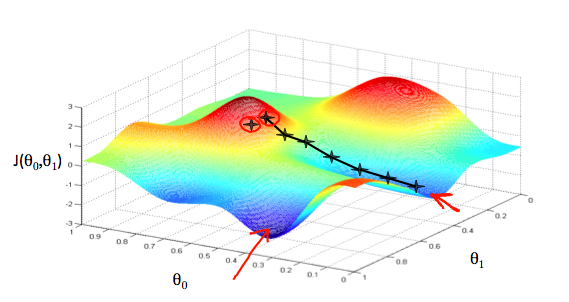
\includegraphics[scale=0.5]{Images/gradiente_descendente.png}

Também poderiamos visualizar o gráfico acima utilizando Contour Line, onde os locais de maior estariam em vermelho e os locais mínimos estariam em azul (igual às cores atuais do gráfico, porém vista de cima - eliminando a necessidade do 3D).

No gráfico podemos ver que dependendo do ponto de inicial dos nossos parâmetros podemos acabar em pontos mínimos diferentes.

Para medirmos o desempenho do nosso treinamento podemos plotar o valor de $C$ a cada iteração para vermos se ela está decrescendo conforme o esperado. Caso a curva do gráfico esteja crescendo significa que o learning rate está muito alto. Se a curva estiver em forma de ondas também significa que está muito alto. Se a curva do gráfico estiver em queda constante significa que o learning rate está bom mas ainda pode melhorar. Se a curva tiver em queda alta e depois diminir a inclinação significa que está num ótimo valor.

Um dos desafios da aplicação do gradiente descendente consiste no fator de termos que calcular o gradiente descendente de cada entrada de treino (para cada input \emph{x} precisamos calcular o $\nabla C_x$ e, então, calcular a média conforme $\nabla C = \frac{1}{n}
\sum_x \nabla C_x$. Tendo uma grande quantidade de entrada para treinamento o aprendizado poderá ocorrer de forma muito lenta.


\subsubsection{Stochastic Gradient Descent}
Para contornar este problema podemos utilizar o \emph{stochastic gradient descent} onde esses passos são feitos em \emph{mini-batch} divididos aleatóriamente a partir da amostra para treinamento.
Esses mini-batches são gerados e utilizado para treino várias vezes (uma para cada época -\emph{epoch}), pois a cada mini-batch fazemos uma alteração dos parâmetros e tendo \emph{epoches} permitirá que uma alteração do último mini-batch tenha um dado menor daquelas feitas após o primeiro mini-batch.

Com um mini-batch de tamanho \emph{m} e o tamanho total dos dados é \emph{n}, teremos:
\[
  \frac{\sum_{j=1}^m \nabla C_{x_{j}}}{m} \approx \frac{\sum_{j=1}^n \nabla C_{x_{j}}}{n} = \nabla C
\]

E nossas variáveis serão calculadas conforme:
\[
  weight \rightarrow w' = w-\frac{\eta}{m}
  \sum_j \frac{\partial C_{x_j}}{\partial w}
\]
\[
  \emph{bias} \rightarrow b' = b-\frac{\eta}{m}
  \sum_j \frac{\partial C_{x_j}}{\partial b}
\]

Estamos dividindo $\eta$ por \emph{m} pois estamos efetuando o aprendizado em mini-batches. As vezes não teremos o tamanho exato do mini-batch, então não precisaremos dividir.


\subsubsection{Normalização}
Dependendo dos nossos dados a convergência para o local mínimo no gradiente descendente pode ser muito lento, isto acontece particulamento quando a escala de valores das nossas features (valores do input \emph{x}) são diferentes.
Exemplo, o input $x_1$ tem valores entre 0 e 2000 enquanto $x_2$ tem valores entre 0 e 5, neste caso o nosso gradiente descendente pode gerar um Contour Line muito fino, o que causa uma convergência muito lento (será feito muito zig-zag dependendo do ponto de inicialização), conforme a imagem.\\

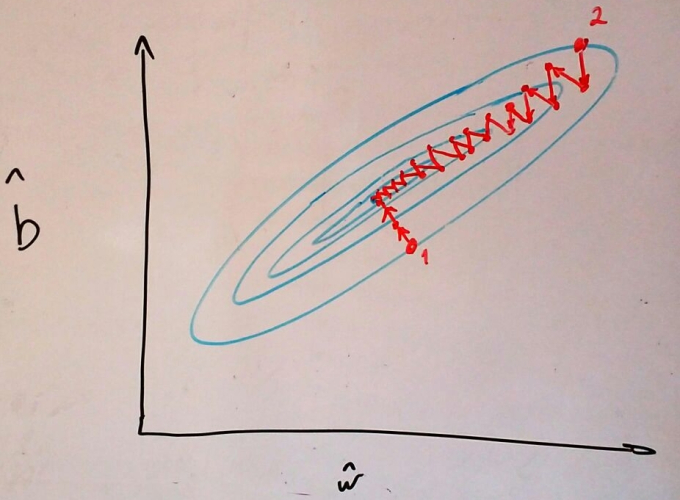
\includegraphics[scale=0.3]{Images/gradiente_descendente_contour_ruim.jpeg} 

O idela é utilizarmos features com escalas similares para que o Contour Line fique com o seguinte formato:\\
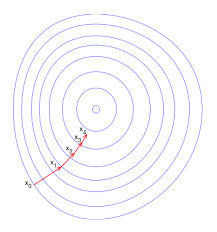
\includegraphics[scale=0.5]{Images/gradiente_descendente_contour_ideal.png} 

Essa escala seria em torno de $-1 \leq x_i \leq 1$ ou alguma outra escala com valores próximos.
Podemos normalizar nosso input fazendo um \emph{scaling} dos dados utilizando duas estratégias: dividindo pelo range dos valores ou aplicando normalização média.
\\

\textbf{Feature Scaling}\\
Para cada feature do nosso input \emph{x} aplicamos a divisão da feature pelo su range, conforme a seguinte fórmula:
\[
x_i = \frac{x_i}{R_i}
\]
onde R é o range dos valores cálculado conforme: $R_i =$ \emph{valor máximo - valor mínimo} da feature no dataset.
\\

\textbf{Normalização Média}\\
Para cada feature do nosso input \emph{x} subtraímos o valor médio da feature no data set, conforme:
\[
x_i = x_i - \mu_i
\]
onde $\mu_i$ é o valor médio da feature $i$ do dataset.
\\

\textbf{Normalização Média e Feature Scaling}\\
Podemos aplicar ambas as técnicas conforme:
\[
x_i = \frac{x_i - \mu_i}{Sd_i}
\]
onde $\mu_i$ é o valor médio da feature $i$ do dataset, $Sd_i$ é o range (valor máximo - valor mínimo) ou o desvio padrão da feature do dataset.



\subsubsection{Regularização}
Em alguns momentos, nosso modelo pode acabar se tornando \emph{overfit} ou \emph{high variance}, quando ele prevê tão bem os testes mas não generaliza corretamente, ou seja, está viciado nos testes.

Para resolver/evitar o \emph{overfit} podemos:
\begin{itemize}
\item Reduzir o número de features - pois a quantidade está causando a grande variação que permite se encaixar exatamente nos dados de testes
\item Regularizar os parâmetros - adicionar um custo nos parâmetros de cada feature
\end{itemize}

Ao aplicar a regularização dos parâmetros $\Theta$ adicionamos um custo neles.
Nossa função de custo fica no seguinte formato:
\[
Minimizar \ \Theta \rightarrow C (\Theta) = \frac{1}{2m} \sum_{i=1}^m ( h_\theta (x^{(i)}) - y^{(i)}) ^ 2 + \lambda \sum_{j=1}^n \theta_j^2
\]
onde $\lambda$ é o parâmetro da regularização que define o custo para os parâmetros, ela causará uma variação no valor dos parâmetros durante o treinamento.

Se $\lambda$ for muito grande pode causar um underfit (pois $h_\theta (x) \approx 0$. Se for muito baixo não causa nenhuma diferença (como se não houvesse regularização pois o custo poderá ser 0).\\


\textbf{Regressão Linear Regularizada}
Para aplicar regulizarização na Regressão Linear precisamos atualizar os parâmetros no gradiente descendente da seguinte forma:
\[
\theta_j := \theta_j - \alpha	 \left[ \frac{1}{m} \sum_{i=1}^m ( h_\theta(x^{(i)}) - y^{(i)})x_j^{(i)} + \frac{\lambda}{m} \theta_j \right]
\]
onde $\frac{\lambda}{m} \theta_j$ é o termo que regulariza nosso parâmetro $\theta_j$.
Podemos reescrever como:
\[
\theta_j := \theta_j (1 - \alpha \frac{\lambda}{m}) - \alpha	 \frac{1}{m} \sum_{i=1}^m ( h_\theta(x^{(i)}) - y^{(i)})x_j^{(i)}
\]
onde $1 - \alpha \frac{\lambda}{m} < 1$ pois este termo regulariza o $\theta_j$.


\subsection{Backpropagation}
Para podemos efetuar a atualização dos nossos \emph{weigths} e \emph{biases} considerando o erro calculado com a função de custo $C$ podemos utilizar a técnica chamada backprograpation.

O algoritmo consiste em calcular o erro da NN com uma função de custo escolhida, este erro é o erro da camada de output do NN. Tendo o valor do erro de cada neurônio da camada de output podemos efetuar a prograpação do erro para as camadas anteriores para que cada neurônios nessas camadas efetuem as atualizações de seus weights e biases conforme seus erros.

Podemos visualizar o processo de encontrar o erro na função de custo e segui-lo até um determinado neurônio onde a mudança em seu weight causou várias mudanças nas camadas seguintes.

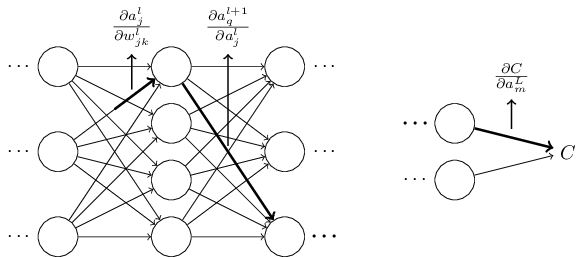
\includegraphics[scale=0.5]{Images/backpropagation_delta_w_effect.png} 

\subsubsection{Erro da Camada de Output}
Utilizando a função de custo $C$ com os parâmetros e outputs da camada de output da NN podemos obter o erro $\delta$ nossa NN.

Uma rede com $L$ camadas podemos calcular o erro do seu output (soma do erro de cada neurônio da camada de output $L^{th}$) usando:
\[
C = \frac{1}{2} \sum_j (y_j - a^L_j)^2
\]

Para calcular o erro de um neurônio $j^{th}$ de uma camada $L^{th}$ usamos:
\[
C^L_j = \frac{1}{2} (y_j - a^L_j)^2
\]
onde $y_j$ é o output esperado do neurônio e $a^L_j$ é o output atual (ativação) dele.

Sendo $a^L_j = \sigma(z^L_j)$ e $z^L_j = w^L_j a^{L-1} + b^L_j$, podemos definir a varição do erro em função do seu \emph{weighted input} $z$:
\[
	\delta^L_j = \frac{\partial C}{\partial z^L_j}
	= \frac{\partial C}{\partial a^L_j} \frac{\partial a^L_j}{\partial z^L_j}
	= \frac{\partial C}{\partial a^L_j} \sigma'(z^L_j)
\]
onde a parte $\frac{\partial C}{\partial a^L_j}$ mede a taxa de variação em função da ativação do neurônio $j^{th}$ e $\sigma'(z^L_j)$ mede a taxa de variação em função do \emph{weighted input} $z^L_j$. Simplificando, pegamos a taxa de variação do erro em função da ativação e multiplicamos pela taxa de variação da ativação em função do \emph{weighted input} para sabermos o quanto o erro varia em função de $z$, pois com ele podemos saber a influência do weight e bias no erro do neurônio.

Nota: A forma exata dessas duas partes variam conforme a função de custo e a função de ativação escolhidas (aqui no caso foram escolhidas Mean Square Error e sigmoid).

O erro definido por $\delta^L_j$ é referente a um neurônio $j^{th}$ da camada $L^{th}$. Para calcularmos o $\delta$ para todos os neurônios da camada $L^{th}$ usamos:
\[
	\delta^L = \nabla_a C \odot \sigma'(z^L)
\]
onde $\nabla_a C$ é o vetor de $\frac{\partial C}{\partial a^L_j}$, ou seja, o vetor com as taxas de variação em função da ativação de cada neurônio da camada $L^{th}$.

No caso da função de custo Mean Square Error, temos a derivada de $C$ em função de $a$:
\[
	\frac{\partial C}{\partial a^L_j} = a^L_j - y_j
\]
Sendo $y$ o vetor de output esperado da camada $L^{th}$:
\[
	\nabla_a C = a^L - y
\]
Então podemos definir o erro $\delta^L$ como:
\[
	\delta^L = (a^L - y) \odot \sigma'(z^L)
\]
Nesta forma todos os componentes são vetores, logo podemos implementar utilizando libs de operações em matrizes e vetores.

Com isso, temos o erro de cada neurônio da camada $L^{th}$ da NN (camada de output). Agora podemos efetuar a propagração desse erro para as camadas anteriores para que cada camada efetue o ajuste necessários nos seus parâmetros (\emph{weights e biases}).

\subsubsection{Prograpação do Erro para Camada Anterior}
Sabendo o erro de uma camada podemos calcular o erro da camada anterior ao pegar o erro e multiplicar pelo vetor de weights transposto. Fazendo isso estamos propagando o erro levando em conta o peso de cada conexão do neurônio.

Tendo esse erro propagando já considerando os pesos, podemos multiplicá-lo pela derivada da função de ativação para descobrirmos o erro em função do \emph{weighted input} da camada anterior.

Esses dois passo é expresso na fórmula:
\[
	\delta^l = \left( (w^{l+1})^T \delta^{l+1} \right) \odot \sigma'(z^l)
\]

Com a função para calcular erro de uma camada anterior e a função para calcular o erro a partir da camada de output podemos calcular o erro de qualquer camada.


\subsubsection{Variação do Custo em Função do Bias}
Podemos considerar que o erro de um neurônio tenha sido causado pelo valor do seu bias.
Assim, podemos definir:
\[
	\frac{\partial C}{\partial b^l_j} = \delta^l_j
\]
Qualquer variação no bias causará uma variação no erro com o mesmo valor.


\subsubsection{Variação do Custo em Função do Weight}
Podemos calcular a variação em relação ao weight usando:

\[
	\frac{\partial C}{\partial w^l_{jk}} = a^{l-1}_k \delta^l_j
\]
Conforme $a^{l-1}_k$ se aproxima de 0, o $\frac{\partial C}{\partial w^l_{jk}}$ também irá se aproximar, exceto nos casos em que o erro $\delta^l_j$ seja muito alto.
Com a variação se aproximando de 0, a mudança no valor do weight após a propagação será bem pequena, nesse caso dizemos que o aprendizado é lento pois a mudança foi bem pequena.



\subsubsection{Algoritmo Completo}
As equações do backpropagation nos fornece uma maneira de calcular o gradiente descendente de uma função de custo para um input do dataset de treinamento.

Abaixo seguem os passos do algoritmo para um input x:
\begin{enumerate}
\item Input $x$: definir a ativação correpondente $a^1$ para a camada de input;
\item Feedforward: para cada $l = 2, 3, ..., L$ calcular $z^l = w^l a^{l-1} + b^l$ e $a^l = \sigma(z^l)$;
\item Output error: calcular o vetor $\delta^L = \nabla_a C \odot \sigma'(z^L)$;
\item Backpropagate error: para cada $l = L-1, L-2, ..., 2$ calcular $\delta^l = \left( (w^{l+1})^T \delta^{l+1} \right) \odot \sigma'(z^l)$;
\item Output: gradiente da função de custo é dado por $\frac{\partial C}{\partial w^l_{jk}} = a^{l-1}_k \delta^l_j$ e $\frac{\partial C}{\partial b^l_j} = \delta^l_j$.
\end{enumerate}

Na prática, é comum combinar o backpropagation com algum algoritmo de aprendizado como o Stochastic Gradient Descent, onde é calculado o gradiente descendente para um conjunto de inputs do dataset de treinamento.

Abaixo seguem os passos do algoritmo para um mini-batch com $m$ inputs:
\begin{enumerate}
\item Definir os inputs do mini-batch
\item Para cada input $x$ do mini-batch: definir correspondente ativação $a^{x,1}$ e efetuar os passos:
\begin{itemize}
\item Feedforward: para cada $l = 2, 3, ..., L$ calcular $z^{x,l} = w^l a^{x,l-1} + b^l$ e $a^{x,l} = \sigma(z^{x,l})$;
\item Output error: calcular o vetor $\delta^{x,L} = \nabla_a C_x \odot \sigma'(z^{x,L})$;
\item Backpropagate error: para cada $l = L-1, L-2, ..., 2$ calcular $\delta^{x,l} = \left( (w^{l+1})^T \delta^{x,l+1} \right) \odot \sigma'(z^{x,l})$
\end{itemize}
\item Gradiente descendente: para cada $l = L,L-1,...,2$ atualizar os weights conforme $w^l \rightarrow w^l-\frac{\eta}{m} \sum_x \delta^{x,l} (a^{x,l-1})^T$ e os biases conforme $b^l \rightarrow b^l-\frac{\eta}{m} \sum_x \delta^{x,l}$
\end{enumerate}



\newpage
\section{Links e Referências}
\begin{itemize}
\item https://spin.atomicobject.com/2014/06/24/gradient-descent-linear-regression/
\item http://www.willamette.edu/~gorr/classes/cs449/momrate.html
\item http://www.asimovinstitute.org/neural-network-zoo
\item http://karpathy.github.io/neuralnets/
\item https://www.ics.uci.edu/~fielding/pubs/dissertation/top.htm
\item http://www.deeplearningbook.org/
\item http://neuralnetworksanddeeplearning.com/
\item https://matheusfacure.github.io/tutoriais/
\item https://chrisalbon.com/
\item https://www.coursera.org/learn/machine-learning
\end{itemize}





\section{Artigos para ler}
\begin{enumerate}
\item One-Shot Learning with Memory-Augmented Neural Networks \linebreak (https://arxiv.org/pdf/1605.06065.pdf)
\end{enumerate}


\end{document}
